\documentclass[openright]{report}
\usepackage[utf8]{inputenc}
\usepackage[table]{xcolor}
\usepackage{fancyhdr}
\usepackage{extramarks}
\usepackage{amsmath}
\usepackage{amssymb}
\usepackage{flafter} 
\usepackage{amsthm}
\usepackage{multicol}
\usepackage{amsfonts}
\usepackage{tikz}
\usepackage[plain]{algorithm}
\usepackage{forest}
\usepackage{algpseudocode}
\usepackage{changepage}
\usepackage{siunitx}
\usepackage{wasysym}
\usepackage{mathtools}
\usepackage{titlesec}
\usepackage{indentfirst}
\usepackage{graphicx}
\usepackage{titletoc}
\usepackage{array}
\usepackage[toc,page]{appendix}
\usepackage[hyphens,spaces,obeyspaces]{url}
\usepackage{tabulary}
\usepackage[labelformat=empty]{caption}
\usepackage[english]{babel}
\usepackage[nottoc]{tocbibind}
\usepackage{chngcntr}
\counterwithout{figure}{chapter}
\usepackage[T1]{fontenc}
\usepackage{listings}
\usepackage{xcolor}
\usepackage[scaled=.85]{beramono}

\newcolumntype{K}[1]{>{\centering\arraybackslash}p{#1}}

\graphicspath{ {images/} }
\usetikzlibrary{automata,positioning}

\usetikzlibrary{shapes.geometric, arrows}

\tikzstyle{startstop} = [rectangle, rounded corners, minimum width=3cm, minimum height=1cm,text centered, draw=black, fill=red!30]
\tikzstyle{io} = [trapezium, trapezium left angle=70, trapezium right angle=110, minimum width=3cm, minimum height=1cm, text centered, draw=black, fill=blue!30]
\tikzstyle{process} = [rectangle, minimum width=3cm, minimum height=1cm, text centered, text width=3cm, draw=black, fill=orange!30]
\tikzstyle{decision} = [diamond, minimum width=3cm, minimum height=1cm, text centered, draw=black, fill=green!30]
\tikzstyle{arrow} = [thick,->,>=stealth]

\renewcommand{\familydefault}{\rmdefault}

\topmargin=-0.45in
\evensidemargin=0in
\oddsidemargin=0in
\textwidth=6.5in
\textheight=9.0in

\linespread{1.25}

\pagestyle{fancy}

\renewcommand{\chaptermark}[1]{\markboth{#1}{}}

\lhead{\projectAuthorShort}
\chead{\reportTopic}
\rhead{\leftmark}
\lfoot{\lastxmark}
\cfoot{\thepage}

\newcommand{\reportTopic}{Phase I and II Report}
\newcommand{\projectAuthorShort}{Cybersecurity Education Group}
\newcommand{\projectTitle}{Hands-on Cybersecurity Education}
\newcommand{\reportDueDate}{February 23, 2018}
\newcommand{\reportClass}{Synthesis Design II}
\newcommand{\reportClassInstructor}{Professor Dana Elzey}
\newcommand{\reportAuthorName}{Clark Benham (cb5ye), Calvin Krist (czk4ja), Saeed Razavi (slr4gf),\\and Jake Smith (jts5np)}
\newcommand{\collaborators}{}

\title{
    \vspace{2in}
    \LARGE{\textbf{\projectTitle}}\\
    \vspace{0.1in}\large{\reportClass:\ \reportTopic}\\
    \vspace{0.1in}\large{\reportClassInstructor}\\
    \normalsize\vspace{0.1in}\large{Due\ on\ \reportDueDate\ at 5:00pm}
    \vspace{1.4in}
}

\author{\reportAuthorName}
\date{}

\renewcommand{\contentsname}{Table of Contents}
\titlespacing*{\chapter}{0pt}{-40pt}{40pt}

\titleformat{\chapter}
  {\Large\bfseries} % format
  {}                % label
  {0pt}             % sep
  {\huge \vspace{-0.2in}}           % before-code

\begin{document}

\maketitle

\large{\tableofcontents}

\chapter{Background}

\section{Introduction}

\par Software is ubiquitous in many countries today. Companies use software to manage user data and offer services. Consumers use it to work, relax, and learn about the world. It's used by governments to help manage elections, recognize citizen needs, and protect their sovereignty. 

\par Software is also used for malicious purposes: criminals, both organized and free-lance, use software, called `malware', to attack businesses, consumers, and governments for personal gain. Malware is also used by activists such as Anonymous to damage those they view as harmful, such as their attack against the World Trade Organization\cite{anonymous_attack}. Even governments use malware for unethical purposes: the NSA's PRSIM program was discovered to be conducting warrantless surveillance on U.S. citizens\cite{nsa_illegal}. High quality programs that costs millions to produce have been used to destroy infrastructure and attack nation states, such as Stuxnet, believed to have been made by the United States\cite{stuxnet}. Autocratic regimes, such as that in Lebanon, use malware to spy on their own people and attack political dissidents\cite{lebanon}.

\par In order to combat malicious software, a specialized security field called `cybersecurity' arose that protects software systems and responds to attacks through a variety of means. Cybersecurity professionals from Gartner, an IT research company, defined the term as "security practices related to the combination of offensive and defensive actions involving or relying upon information technology and/or operational technology environments and systems"\cite{cyber_def}. In other words, the field of cybersecurity encompasses both attacking and defending systems such as computers, networks, and databases. Due to the components of these systems, cybersecurity professionals are often also called IT security professionals. This field is taught at many universities today, and cybersecurity professionals are in high demand from both companies and governments due to the extreme integration of software into modern society, the high value of user data, and a lack of qualified professionals.

\section{Market Need}

\par At the most superficial level, malware hurts the economy and people's lives. Cyber attacks cost the global economy \$400 billion annually, and is only increasing. This cost largely comes from stealing user data, such as credit cards and medial information, and by shutting down company infrastructure. There are thousands of such attacks world-wide: in 2016, there was over 1000 data breaches of U.S. companies alone. For example, Maersk, the shipping company, had all their computer systems infected by ransomware (malware that stops the user from doing anything until they pay a fee). This completely halted their operations for over a week as they switched back to pen-and-paper management and quickly rebuilt all their servers and databases from the ground up. This attack, which did not even target the company, cost them about \$250 million\cite{maersk}. Another example comes from 2017, when Equifax was hacked, exposing the personal data of over 160 million Americans - data that included credit card numbers, social security numbers, and more. This allows criminals to steal people's identity and conduct all types of fraud.

\par It should be noted that it's not always the economy or individuals who are hurt: political systems and entire cultures can be damaged as well. For example, Russia's hacking of the elections compromised the integrity and sovereignty of the United States\cite{russa_indicement}. The operations consisted largely of leaking DNC emails and an extensive online disinformation campaign on social media, disguising the foreign influence through special servers and long-term user accounts\cite{russa_indicement_nyt}\cite{what_russia_did}. This is a corruption of the democratic culture, and could have long term effects both nationally and internationally. 

\par Autocratic regimes, or even those with a less democratic culture than the United States, often use surveillance software (spyware) to spy on political dissidents and journalists trying to report on 'politically harmful' information. As a result, many companies sell 'security solutions' to autocratic regimes such as Ethiopia which are used to spy on their citizens\cite{ethiopia_surveillance}. Mobile devices can be turned into tools of repression, where messages one sends to others expressing dissatisfaction can be means for arrest or other forms of retaliation. Countries like Saudi Arabia own large shares in infamous cyber security companies like Hacking Team and use their products for espionage on their own citizens\cite{saudi_cyber}. Mexico illegally uses hacking tools to spy on activists and reporters in order to intimidate and harass them\cite{mexico_cyber}. In other words, malware is actively used to support autocratic and politically harmful practices.

\par Part of this excess of cyber attacks and malware comes from the fact that IT security professionals have to defend entire systems that have hundreds of vulnerabilities, while attackers have to find just one weak point. In other words, attacking is inherently easier than defending. However, there also aren't enough qualified cybersecurity professionals for all the businesses and governments in any country, leaving user data vulnerable to attack. 90\% of companies worldwide say they are unprepared for cyber attacks, and governments similarly have trouble. 70\% of U.S. federal IT security professionals say the government lacks qualified employees, and 86\% say they have trouble finding personal to fill spots\cite{fed_cs_jobs}. It is estimated that, by 2020, there will be 1.5 million unfilled cybersecurity jobs in the U.S., leaving the way open for user data and companies to be more vulnerable than ever\cite{why_no_cyber_classes}.

\par The direct cause of this issue can be seen in a report made by the ISACA in 2017, an international association of IT professionals. They surveyed members of their association and found that most IT security job posting just get around 5 responses, and only around 10\% of job postings get at least 20 responses. In contrast, most corporate job openings receive between 60 and 250 applicants\cite{job_survey}. This is because \textit{everyone} needs IT security professionals, and there are not enough of them to go around.

\par This problem is further compounded by the fact that few of those who even respond to cybersecurity job postings are qualified: the ISACA found in their survey that nearly half of those questioned said that one in four of respondents to their job posting are qualified. The number one reason potential hires were unqualified was a lack of hands one experience\cite{job_survey}. In other words, not only do very few people respond: an astounding proportion of respondents are un-hireable. This leaves the whole world without the necessary number of cybersecurity experts to protect them.

\section{Observations}

\par In order to fully understand the problem, we approached the problem in a few different ways. In addition to the online research mentioned in the other sections, we spoke directly with a range of students and professionals about their experiences with cybersecurity. Novices to cybersecurity with whom we spoke expressed feelings of ignorance about the field, with some expressing anxieties about the difficulty of starting an education in the discipline. This included people we know to be talented at computer science in general, such as Rodmans who chose to work on other projects to avoid cybersecurity. We also discussed the topics with more experienced students in the Cyber Defense Team and the Network Security club. The general sentiment expressed was that, like the novice students had lamented, it was very difficult for each of them to make their way into the field with those who had been introduced to it in the context of the groups having the most success in overcoming the barrier to entry. They expressed generally that it was much easier to further their education once actually in a community which promoted and taught cybersecurity education. 

\par The primary industry professional with whom we spoke was Professor Ibrahim. We had an hour long interview with him about the types of labs he does and the difficulties he has implementing them. Many students, we learned, have very small amounts of RAM and have trouble running the required software. Furthermore, because he mostly does network security labs, he is limited by the number of routers he can procure. Finally, when a single student has trouble with the lab he has to choose whether to help the student debug the problem, forcing the other 50-80 people to wait, or to move on without the student\cite{ibrahiminterview}.

\par We have also observed how cybersecurity classes are taught at MIT graduate programs through the MIT open course ware. They don't have adversarial labs, nor do they interact with real world systems: instead, they analyze carefully crafted pieces of code and study vulnerabilities from a theoretical perspective. This shows that issues with hands-on experience are not localized to UVA and extend even to the highest tier of education\cite{mit}.

\section{Problem Identification}

\par Why are there so few cybersecurity job applicants and why are so few of them qualified? To begin, this is a very new field. As a result, there is no consensus as to what students should be taught and how they should be taught\cite{why_no_cyber_classes}. This means that there can be a large discrepancy between what employers want, what employers need, and what students are taught. Furthermore, not many universities offer undergraduate degrees in cybersecurity, much less a quality education in the field. This includes the University of Virginia. Here at UVA, there is currently a lot of debate between CS professors as to how much security education should be required to get a degree\cite{ibrahiminterview}. Currently, while numerous security courses are offered and more are coming, there is no requirement to take one\cite{comsci_handbook}. Students only study cybersecurity if it interests them.

\par This results in two things: normal software developers leave more vulnerabilities in their applications, and less students become interested in cybersecurity. Not teaching basic security to CS undergraduates means that those students, now professional developers, are not aware of the security needs of applications or the ways that they can expose user data. This means lots of software, much of which is used by consumers, have vulnerabilities that can be abused by malicious hackers\cite{why_no_cyber_classes}. If graduates were required to take basic security courses, they may be more cognizant of the security of their applications and consumers would be safer.

\par Furthermore, many students will not take cybersecurity courses unless it is required. Cybersecurity, in contrast to most of computer science, is very intimidating. It has a dry reputation, and it's generous to say that there even \textit{basics} to cybersecurity. As we have seen by talking with students, many don't know where to begin studying the topic. 

\par Cybersecurity requires vast domain experience due to the diversity of systems that need to be protected. As a result, it's hard to learn and hard to become passionate about because there is no immediate payoff to studying it. This means that few students will become interested in the field on their own, and without universities pushing students towards towards the field, this problem will not be rectified.

\par Even for those who decide cybersecurity is a topic worth pursuing, there are many barriers. Much of cybersecurity is about the interaction of systems. This means that to do more than read about topics--to get hands on experience--students need to be able to set up or simulate the systems they read about. Students need to know more than just intermediate programming and network theory: they also need to be server experts, OS experts, and knowledgeable about service architecture. 

\par This asks a lot of students. The necessary complexity of these systems makes them difficult to set up, and even following an online tutorial is frustrating. Small differences in computer configurations can result in hours of hard work debugging the problem. This is very discouraging, and can slow down student learning or even dissuade them from the field entirely. 

\par These same problems are why many university graduates lack hands on experience and are unqualified for most IT security jobs. Because of the nature of teaching in a classroom, the labs have to work for all students. If the lab doesn't work on one student's computer, the professor is faced with a painful decision: to leave the student behind, or hold up the whole class to try and debug the issue. As a result, most labs are as simple as possible while still demonstrating core concepts to reduce the time spent setting up and the risk of a student not being able to participate\cite{ibrahiminterview}. This means that, for universities to give students hands on experience, the best technology right now is to have dedicated computer labs set up for students to use. A computer for every student, enough routers and servers for all of them, the databases necessary. This would be incredibly expensive, take lots of time to set up, test, and prepare, and it still could fail.

\par The result is that schools can't give students hands on experience and students have lots of trouble getting that experience themselves. Thus, most of those that do choose to study this field lack the requisite experience necessary to be a qualified IT security professional.

\begin{center}
    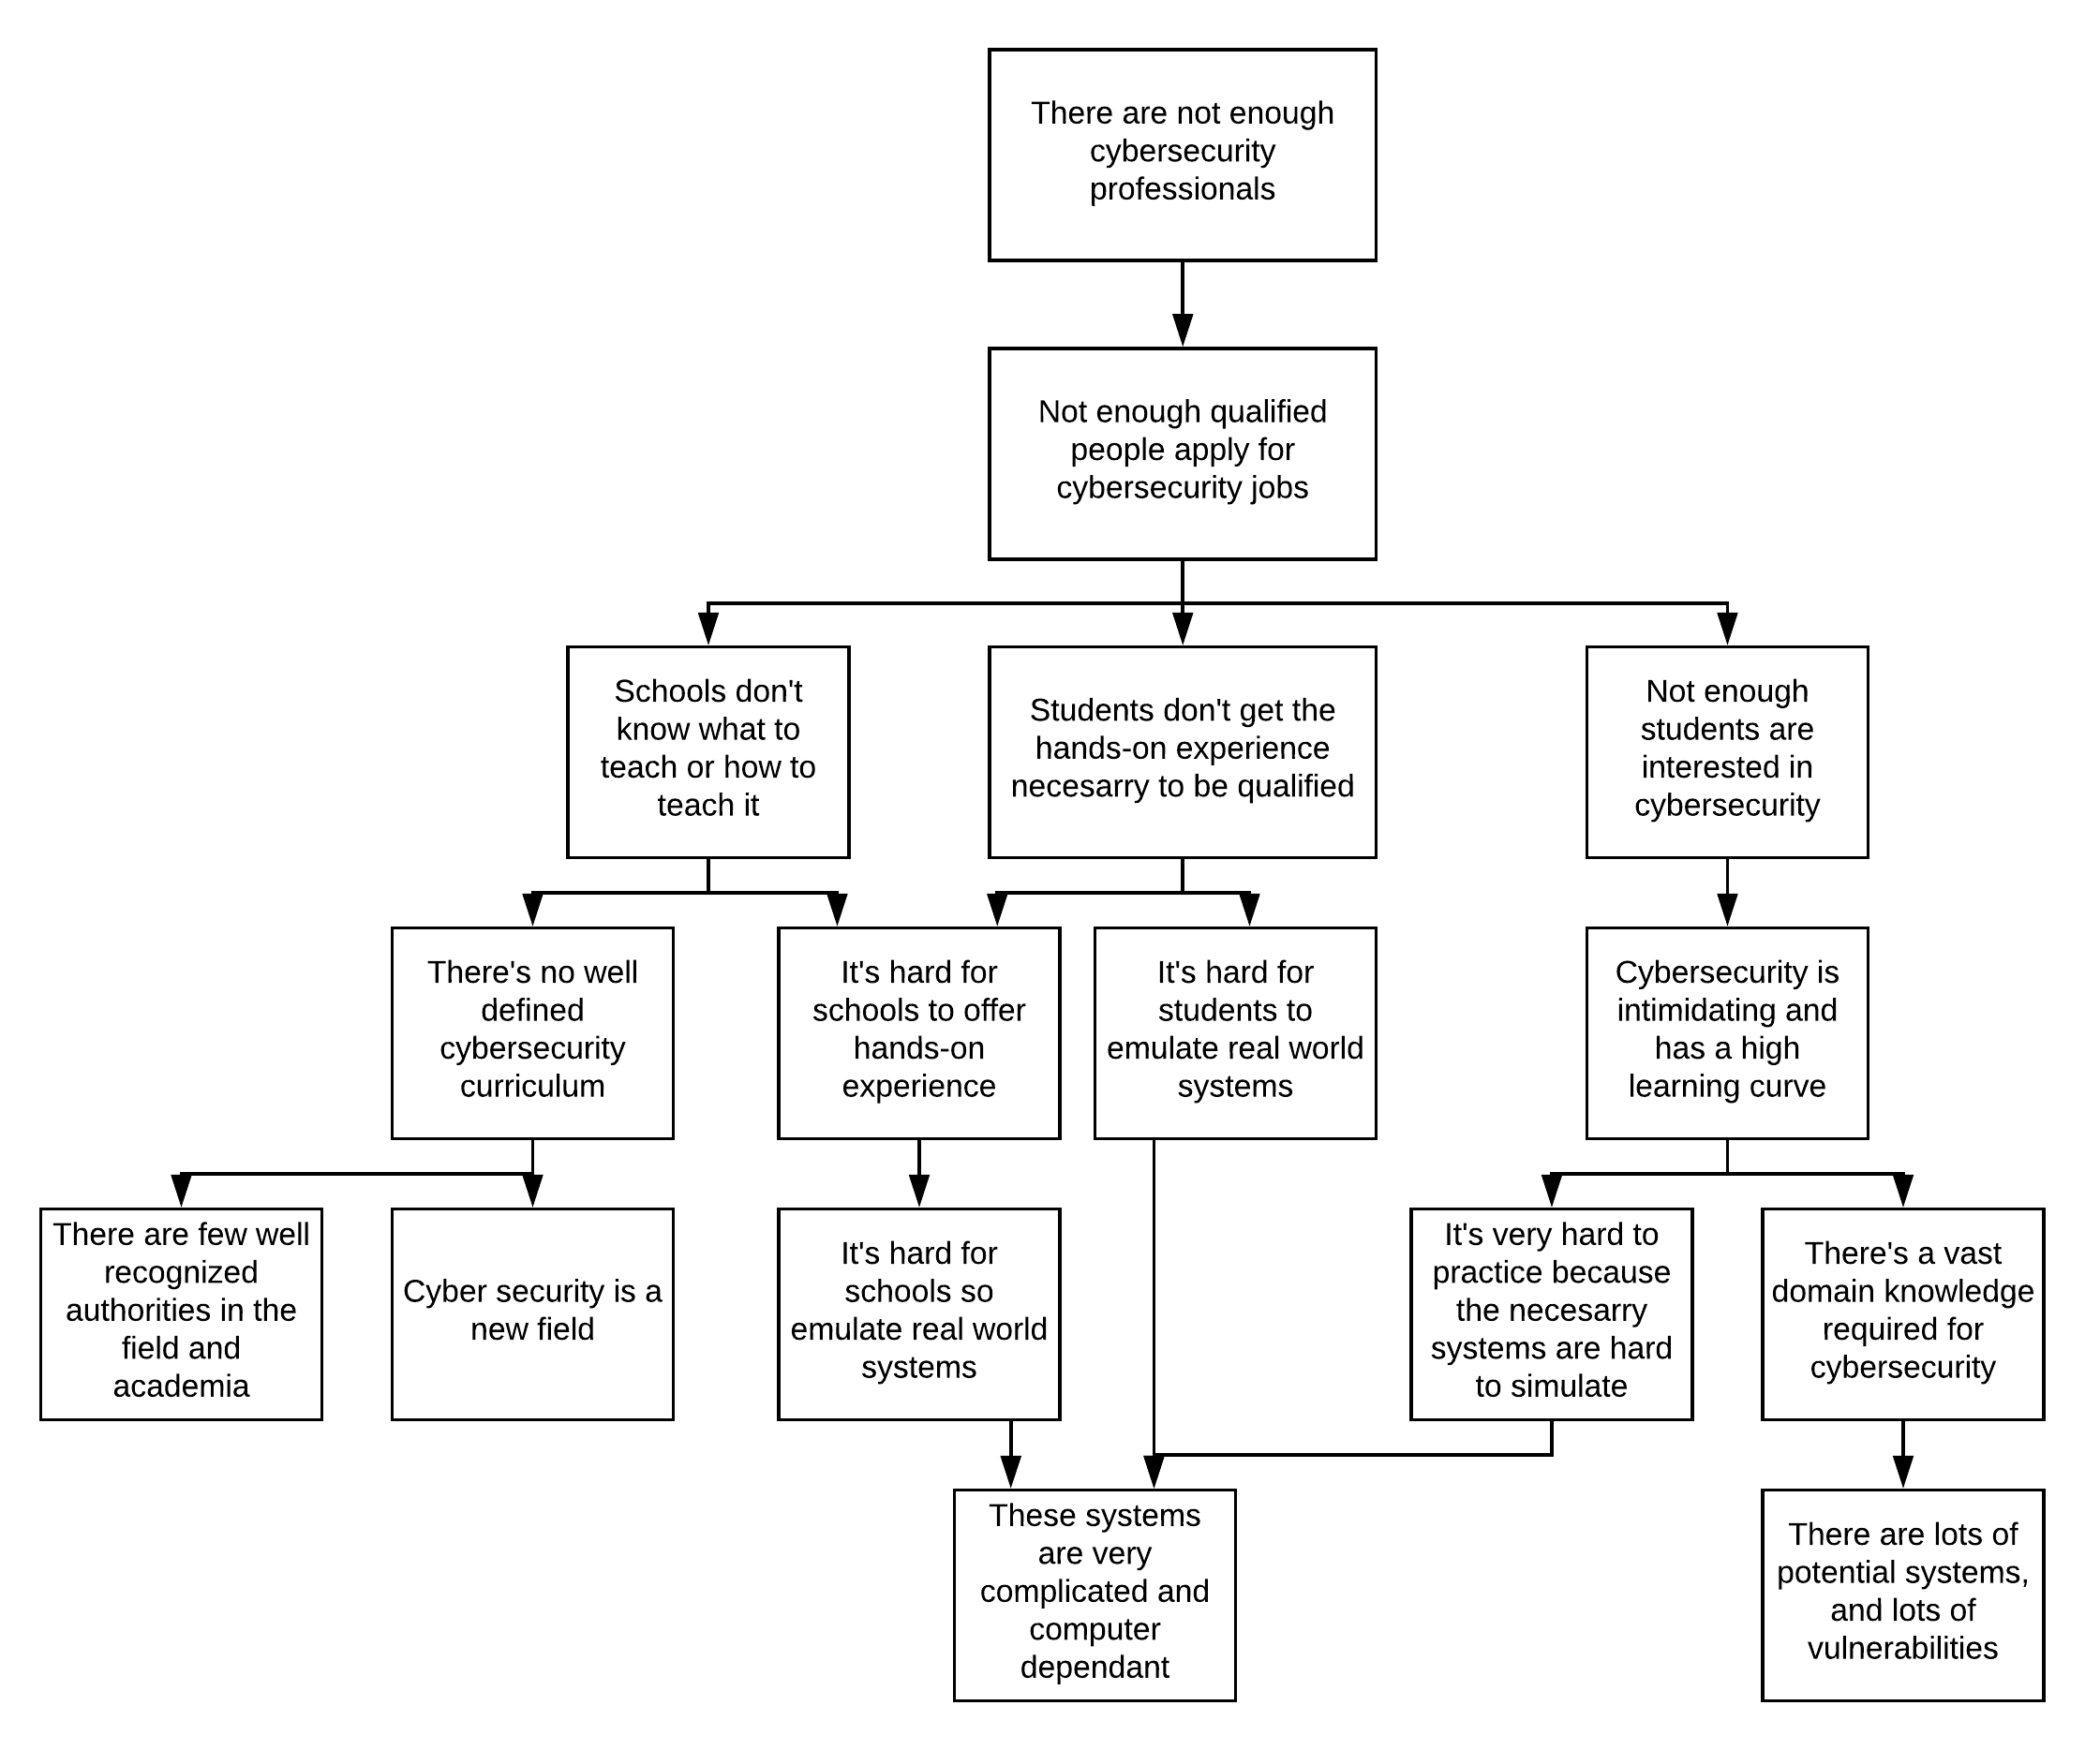
\includegraphics[scale=0.34]{images/Why-Why.png}
    \captionof{figure}{\textbf{Figure \arabic{figure}:} Why-Why Diagram identifying the problem}
\end{center}

\par As can be seen in Figure 1, there are a few different conclusions that can be drawn. As has been discussed, cybersecurity is complicated because the systems it needs to defend are complicated: that can't be changed because the systems serve users. Furthermore, the line of inquiry regarding curricula is currently being worked on by other entities with lots of power, resources, and know-how. Specifically, the NSA developed criteria for measuring academic excellence in cybersecurity departments. Criteria include topics such as specific content to teach, degree of interdisciplinary education, level of faculty involvement and research, and student engagement. Each of the criteria have different methods detailed for proving how well a school meets them. If a school does well enough, their cybersecurity program will be accredited by the NSA\cite{nsa_accred}. 

\par While only 19 schools are accredited at the moment, it includes universities such as Carnegie Mellon and Virginia Tech\cite{nsa_accred_schools}. The NSA is perhaps the only organization that could push such high quality schools to unify their curricula and develop shared, high quality standards. We expect that in future years many more schools will become accredited, including the University of Virginia. 

\par It would be very difficult for us to contribute to this solution. We are not educators, and do not know how curricula are designed. Nor do we have the knowledge or connections to analyze the NSA's criteria and curricula based on those criteria. Comparing those programs to cybersecurity degrees at other schools would involve comparing metrics such as length of time for graduates to find a job, average satisfaction of employers with the graduates, and figuring out how to control for the fact that some schools will offer more extracurricular cybersecurity opportunities than others. 

\par As such, we decided to focus on a problem we have the resources to tackle: the difficulty in modeling real world systems to get hands-on experience with cybersecurity. In order to help us focus on the issue, we defined the problem statement as:

\textbf{It is very difficult for non-experts to learn and practice cybersecurity in a hands-on manner because of the complicated setup required.}

\par Our goal is to enable students to easily create systems that allow them to study cybersecurity. Our hope is that students, teachers, and professionals can use our product to make the field more approachable and increase the number and proficiency of cybersecurity professionals. This could make a dent on the lack of qualified IT security specialists, lessening the risks associated with a world becoming more and more digital.

\section{Prior Art}

\par One of the greatest limitations of simulating these complex systems is how much they need to vary machine to machine. Furthermore, in the real world these systems are set up on multiple, if not thousands, of machines. As a result, for most it is impossible to set up the hardware to perfectly copy the systems.

\par To counter this issue, various technologies have arrose including:
\begin{itemize}
    \item Virtualization, such as VirtualBox
    \item Virtual Machine servers
    \item Specialized labs based on virtualization
    \item Website based education
    \item Tools like Vagrant to simplify virtual machine deployment
\end{itemize}

\par According to VMware, one of the main vendors of this technology, "virtualization is the "process of creating a software-based, or virtual, representation of something"\cite{virtualization_def}. Servers, machines, and even entire operating systems (OSs) can be virtualized. When a computer is virtualized, it is called a 'virtual machine'. Virtual machines allow people to launch an application on their computer and in the window that appears have access to what is essentially another computer. The software that runs the virtual machines is called an embedded hypervisor, and it takes care of communicating between the software (the simulated OS) and the hardware (the physical components of the host machine)\cite{virtualization_comparison}.

\par Virtual machines are often used to simulate other computers, and even entire networks. This allows one computer to, essentially, be many. Furthermore, in an ideal situation the virtual machines can function on \textit{any computer} due to the hypervisor, reducing the effect of machine-specific configuration issues. Microsoft uses special servers and management tools to host virtual machines that their employers can remotely access\cite{ms_virtual_setup}. While this reduces the cost of IT, and would make it easier for students to simulate real world systems, the hardware alone cost thousands of dollars and the complicated network of servers necessary to implement this solution is exactly what we want to avoid.

\par Virtual machine setups have been utilized by many others, as well, due to its vast applicability to computer science. Some sources recommend setting up a simple virtual machine server for about \$800 due to its advantages over hosting VMs (virtual machines) on a host computer\cite{virtual_mch_server}. Other sources take a more approachable strategy and cut out the server but still have a dedicated VM machine\cite{simple_virtual}. Both of these recommend dedicated machines because running VMs is computationally expensive: a normal VM might take 1.5-4 GB of RAM to run. Many computers only have 6-8 GB of RAM, so running a VM can cause serious lag and frustration to the user. 

\par There have been a few labs built on top of virtual machine technology that, ideally, easily allow users to run a command and install specially configured VMs that can be used to study cybersecurity. The DetectionLab, when installed correctly, offers tools for interacting with Metasploit (a popular penetration testing software). The lab also sets up Window servers, domain controllers, and other infrastructure that students struggle with\cite{detection_lab}. However, in our own experience these labs can easily fail. We were unable to install this lab on any of our machines despite repeated attempts, an we have no clue why it failed.

\par There are numerous technologies to interact with virtual machines, such as the VirtualBox API and Vagrant. VirtualBox is the leading provider if free virtualization technology. Their API allows developers to use scripts to interact with Virtual Machines to configure machines, set up services and servers, and connect to virtual networks\cite{vb_api}. Vagrant can help automate this process. It allows developers to specify simple configuration files which users can then run and have machine-generated scripts set up  virtual machines\cite{vagrant}. This simplifies the process of creating specially configured virtual machines for both the developer and the consumer.

\par Others have tried hosting cybersecurity problems on websites in order to avoid the high computational overhead of virtual machines\cite{website_probs}. This allows users to connect to a website and use computational resources owned by someone else. This can also avoid the cost of paying for hardware, assuming the website owners can find another source of income to host the problems. However, there are limits to what students can practice on these systems. It is hard to study networks, firewalls, or attacks due to the necessary security the website operators install. High quality training programs, such as those run by Palo Alto Networks on the Panacademy network, get around these limitations by owning the entire architecture the website runs on. However, in order to afford that, Palo Alto charges lots of money to use their training\cite{palo_alto}. This is a potential resource that universities and companies can use, but one out of reach of most students.

\par Other approaches to solving the problem can be briefly summarized as they are out of the scope and resources of this project. As has already been discussed, efforts are underway to standardize cybersecurity curricula. Other approaches, namely policy approaches undertaken by governments, involve creating 'cybersecurity initiatives' and pouring money into the industry and universities. Obama proposed plans for a \$19 billion dollar cybersecurity initiative, which included \$62 million for funding education\cite{why_no_cyber_classes}. Countries all over the world are investing heavily in cybersecurity by pushing for more education and increasing the budget to pay for security programs.

\chapter{Solution Identification}

\section{Solution Context and Environment}

\par Before diving into specifics regarding potential solution ideas, it is crucial to first understand the context and environment in which our solution will operate.

\par In an economic context, there is currently a very competitive market for educational and technology based software. This competition continues to drive down prices and raise the overall quality of solutions available to the public. Additionally, with the rise of the open source development mentality of the general community, more and more training resources are being created, completely free for anyone to use and modify\cite{open_source}. By making these tools available under the MIT License or similar terms, creators are able to get more people using their tools. This higher adoption rate ultimately helps the creators better achieve their goal: creating a useful tool that adds value for someone in someway.

\par In keeping with this idea, we are also planning to keep our project (or at least the majority of it) open to the public (ie free to use). By opening our project up to more people, we envision two main benefits. First, with more active users of our product, more diverse and extensive feedback will be generated. We can then in turn utilize this feedback to create a higher quality tool that is tailored to even more people's needs. In addition, one of our overarching goals for the project is to, in general, improve cybersecurity education for beginners. Therefore, it follows that with more people using our solution, our impact on the problem area will multiply. By adding any sort of fee to use our product, at least at this point, we think it would be cost prohibitive for our intended userbase.

\par In a socio-cultural context, as we have mentioned before, cybersecurity is a very recent and quickly evolving field. As a result, our solution will need to be modular enough that it can be easily adapted in the future. Our target audience for the project, students and professors, will remain the same throughout the lifespan of the project. As the years pass, new generations of students will be able to use the tool, so it is important that it can and will be updated regularly. In addition, as new software and operating systems are released, we will want to be able to integrate those into our solution. Another key aspect to recognize is that there will be a large influx of new students jumping into cybersecurity. With all of the major headlines about data breaches, hacks, and job openings, more people will be interested in participating in the field. As with the enrollment growth of computer science majors, we expect a similar double digit or better growth rate in cybersecurity focused students. Finally, in order for any tool to gain widespread popularity in today's world, the user experience is crucial. As such, we will need to ensure we are developing a product that provides ample instruction and an intuitive interface to help the users, especially beginners, as they use the product.

\par In a technological context and as referenced in the Prior Art section, the technology needed to simulate complex business environments is finally reaching the real world. In following with Moore's Law, the computers of today are several times more powerful than those of just a few years ago. As a consequence of this, the required hardware for extensive virtualization is reaching mainstream adoption. As we continue to lower the barrier of entry in terms of capital, more and more students will be able to utilize tools such as ours to learn complex cybersecurity topics. From a software point of view, the concept of containerization has also become popular in recent years. With containerization, people, independent of a specific operating system, can run specific software\cite{docker}. This trend, along with virtualization, will enable us to build on the technologies others have to created to allow anyone on any platform to use our tool. With this portability, we expect that it will be easier for more widespread adoption of our solution. For example, if the professor does not need to worry as much about the details of all the students' machines, they can spend more time on creating the actual content for the lesson.

\section{Customers and Resources}

\par Throughout this project, we will be actively consulting with 3 groups of people that will act as the customers for our project. During our Sprint Reviews, we will be meeting with our customers to present our current solution, get feedback, and plan out ideas for future iterations. Customers include UVA students, professors, and industry professionals. This close relationship between the project team and clients will help to ensure that at the end of the semester, our product will be actually used by people. Often school projects die at the due date, but it is our hope that we will end up creating a tool that lives on well past the final grade.

\par Our first of three customers for the project is the University of Virginia's Computer and Network Security Club. During their activities, they have found that getting demonstrations to work on everyone's computer is, quite simply, a nightmare. In addition, they have been reluctant to try to teach more advanced concepts because they would spend more time trying to configure the exercises than focusing on the cybersecurity aspects. One specific subset of the club is the Cyber Defense Team. For their competitions, they need to defend complex, real world business environments. Similarly to the problems faced in the general club, practicing for the competitions has been difficult. Multiple team members have lamented to us about these problems, so we will be working closely with them to find a solution to this problem.

\par Next, we will be working with Vernon McCandlish who is a Sr. Incident Responder at General Electric and Cybersecurity Professor at Utica College. With his domain expertise in both industry and education, he will be able to provide valuable insight to guide the project. Specifically, his years of experience in the cybersecurity field mean he has a solid grasp on what skills students need to be successful. In addition, his experience teaching other students means that he too has faced similar problems regarding lab set up.

\par Finally, we will be working with some cybersecurity professors here at the University. After speaking with them, we found out that one of their major headaches was creating labs for students to learn new skills. Because they often have large classes with a diverse set of students all with different laptops and software, it is challenging for their labs to work for everyone\cite{ibrahiminterview}. With this goal in mind, we will be working with them throughout the semester to find ways that we can make it easier for their students to participate in the labs without the usual problems. In addition, if our tool is able to simulate more complex business environments, they will be able to potentially teach the students new concepts. Often times they are able to solely discuss these complex topics, but because of the set up required, students are not able to get the hands on experience with the environments.

\par From a resources perspective, we plan to utilize many of the tools and software mentioned in the Prior Art section. These tools handle many of the "under the hood" management needed to virtual software across different platforms. Additionally, we will be employing Github for our project. Github enables us to have a shared central repository for all the code in our project as well as track project progress. Since we are using Scrum as our project management methodology, we will be able to take full advantage of Github's built in tools to track issues and tasks during each sprint. Finally, we will be regularly consulting with the aforementioned parties to gather feedback throughout the project lifespan.

\section{Constraints}

\par Next, we analyze the constraints of our solution in terms of both the project and product in order to understand how we may mitigate these issues throughout the semester. We look at these constraints through the lenses of:
\begin{itemize}
    \item Project Risk
    \item Project Resources and Cost
    \item Project Quality
    \item Product Scope
\end{itemize}

\subsection{Project Risks}

\par We have identified two main categories of project risks so far. First, the software performance and capabilities may not be at the level needed to simulate complex environments. Although available tools such as Virtualbox and Vagrant have come a long way over the past couple years, there are still many limitations to using these tools. Since this is a risk we must accept, we plan to proceed forward after conducting even more research to identify the best options. Then, with our sprint guided development, we expect to run into major issues sooner rather than later. Although this may seem counter-intuitive, by "failing faster," we will be able to modify our project to work within the constraints and end up reducing the limitations of a specific program on our overall project. Next, as hinted at previously, the integration and complexity of the tools we will be using is another constraint. Although most of the tools are stable and work well on their own, we expect to combine them in potentially new ways. This complicated tech stack configuration may introduce bugs and unforeseen issues during the project. To combat this problem, we will again attempt to run into the issues as early as possible, so that we may adjust the scope of the project as needed.

\subsection{Project Resources and Cost}

\par From a Resources perspective, the biggest issue will most likely be the distribution of cybersecurity knowledge throughout the team. Each member on the team has significantly different levels of experience working with the various tools in the technology stack and cybersecurity in general. We anticipate these may cause problems particularly with setting expectations. What may be simple to one member may be very difficult for another. In an effort to mitigate this problem, we are following a two folded approach. First, it is the expectation that our team will regularly communicate in our real time GroupMe channel on problems they run into. Then, if another person has seen the problem before, they will be able to provide support as needed. Next, we have set aside a three hour working session each week where we will all meet up in person. During these sessions, since we are co-located, there will be more knowledge transfer between each development team member. Additionally, this time will allow the more experienced members to train the others. 

\par From a hardware perspective, for the most part, each member of the development team already has decent specifications on their computers. However, it may still be helpful to secure additional hardware or upgrade our computers. Not upgrading may potentially slow down development or limit the amount of testing that we can preform at each stage. Since we will not have any other costs associated with the project, we plan to mitigate this risk by budgeting our money towards computer upgrades if needed. All of the software we plan to utilize during the project is free which will allow us to easily work within our cost constraints.

\par We will also need to secure access to as wide a variety of computers as possible for software testing. This will likely involve having the student resources at UVA test the technology and give feedback, as well as using the UVA computing labs. 

\subsection{Project Quality}

\par From a quality perspective, one of the biggest risks we identified is a limited amount of testing. In the traditional waterfall style project management approach, integration between different systems and testing usually happens toward the end of the project. By this point, identified problems can cost upwards of 10x or more to fix when considering the potential rework required. As a result, we quickly understood this to have an incredible negative impact potential on our project. In our anecdotal experience, estimation and testing are often the leading causes of failure in software related projects, so we decided to take an alternate approach. With our decision to employ Scrum throughout the project, we have the opportunity to fail faster as each week we will be coming together to release a new version of our project. In addition, since we will be presenting it to an actual customer (one of the aforementioned groups), they will be able to hold us accountable for developing high quality software. In order to further mitigate this problem, our weekly working sessions will also act as a time for the project team to test integrating the different components on our solution.

\subsection{Product Scope}
In addition to taking a meta approach to analyze the constraints surrounding the project team itself, we also analyzed our product. By researching the context and environment in which our product will live, it led us to several key aspects that our end product must abide by in a sense. 
\begin{itemize}
    \item Low Cost
    \item Machine and Material Apathetic: 
    \item Simple Setup
    \item Low Technical Specifications
    \item Models Real World Systems
    \item Ethical
\end{itemize}

\par The first of these guiding principles is the cost of our product. Since we are completing this project technically for an alternate form of compensation besides money, we have significantly less costs than a business. As a result, we have the opportunity to develop a free product which will enable a wider end user adoption rate. 

\par Next, a good user experience is another important part of the solution we create. Creating a tool that is intuitive for the user will help our target audience more effectively utilize the tool. When considering students and professors who have less time than most to debug technical problems, a strong user experience must be a core focus in our development efforts. This can be done by making the solution apathetic to the machine it's being run on (ie, it will work on everyone's computer), easy to setup, and it can't require a high quality computer. Failures in these fields will drive away users and fail to simplify the process of getting hands-on experience. 

\par Finally, we must produce a product that is able to effectively simulate more advanced, real-world type configurations. This will allow our product to realize its full mission: creating a hands-on experience to teach the next generation of cybersecurity specialists. Quite simply, if our product is not able to be used as an effective training tool, we will not consider the project a complete success. Part of this means that the solution should be material apathetic as well. If it is only good for penetration testing and can't be used to teach software forensics, then it's not meeting its full potential. Another part of this means that the solution shouldn't unduly enable users to attack others, and it should encourage users to hack ethically. We don't want to train more criminals and defeat the purpose of this project.

\section{Brainstorming}

\par The shortage of adequately trained cybersecurity experts warrants various solutions that approach the problem from different angles. Angles considered included: a change in the platform on which students train (to make training more accessible), an analysis and improvement of available cybersecurity curricula, and other more minor solutions aimed at promoting the discipline of cybersecurity and making security technology easier to implement for users. Once a breadth of approaches were considered, a favored subset was targeted for further scrutiny. The remaining approaches were scored in a variety of categories, the scores were summed, and the approach with the highest total was selected for further development. 

\par The approach of changing the platform on which students are trained addresses the fact that setting up environments in which to practice cybersecurity is time consuming, difficult, and acts as a high barrier to starting any sort of training in the discipline. The primary solutions addressed within this approach were to create website-based training and testing platforms, personal machine-based training and testing platforms, or tools and deployable labs for instructors to implement. 

\par A website-based platform would allow users to learn and practice practical applications of cybersecurity online without the need to download and set up local systems. It was formulated that such a concept could be achieved through the use of secure shell (SSH) and remote desktop protocol (RDP) which would allow secure access to systems over the internet wherein the appropriate environment for security training is already set up. Alternatively, users could type directly into a text box answers to different problems. Other ideas within and expanding upon this method that were considered include hosting coding challenges through online systems such as codeshare and the potential for online teaching through specific courses and exercises. 

\par A personal machine-based platform was considered with multiple avenues for execution including downloadable modules that automatically set up environments for specific tutorials, a one-time download system that downloads and installs a system modeling a business environment with certain per-installed attack simulations, and a general framework to combine the two aforementioned avenues. The solution of creating tools and deployable labs for instructors would entail the creation of labs that would be easily deployable regardless of the local operating system of the machines being used. Instructors would be able to use these labs to visualize attacks for their students. Tools and concepts that expand on the general idea include easily deployable centralized networks and servers to manage labs as well as a framework for a player-versus-player scenario of attack/defense systems within a classroom.

\par The approach of analyzing and improving current cybersecurity curricula, referenced also as "curriculum development", aims to solve the cybersecurity expert shortage by standardizing educational needs and filling holes in preexisting education. The first method discussed in considering this approach was the comparison and contrasting what content is included in different curricula and degree programs globally. Furthermore, it was suggested that data could be collected globally to understand the impacts of different foci of study on job security and job effectiveness in the field of cybersecurity. From this idea, it was expanded that detailed communications might be set up with employers in order to determine what specific needs they may have that are being met as well as those which aren't. An alternate proposal suggested the creation of a network of professors and interested professionals to develop a set of standards for cybersecurity curricula.

\par Other smaller scale approaches to the problem were suggested including the outreach and promotion of cybersecurity as well as the specific goal of making cybersecurity more accessible. The outreach and promotion of cybersecurity as a discipline would theoretically increase the number of people going into the field in the long term. Some solutions in this domain include outreach to high and middle schools, the creation of cheap, easy, and hands on labs for high schools and colleges, and the creation of outreach programs to encourage professors to create more adversarial labs. A subcategory of this domain in which a fair number of ideas generated fell was the gamification of cybersecurity. By treating cybersecurity as play, the anxiety of its complexity and difficulty would be reduced as people are drawn to it at younger ages with more enthusiasm. The alternate domain of focusing on making cybersecurity more accessible contains ideas related to making security technology easier to use for the layman and creating more sources for self-education in cybersecurity. The full list of brainstormed ideas can be found in Appendix A: Brainstormed Solution Ideas List.

\section{Solution Identification}

\par Once a breadth of ideas were brainstormed, a specific subset was selected for further scrutiny based on votes from members of the development team. The smaller scale approaches were eliminated in voting and the curriculum development approach was eliminated in further discussion. It was decided that curriculum comparison was unfeasible given the resources and knowledge available to the development team. The remaining ideas after voting and scrutinizing were the approach involving the website-based training platform, personal machine-based training platform, and easy lab and tool development. 

\par To select our final solution, all three were compared in a KTDM chart. This involved rating each idea from zero to ten in a number of categories, each of which were assigned a weight. The weight and rating were multiplied to determine a score for each approach in each category. Then, the scores for each category were summed up to create a total score for each approach and the approach with the highest total was selected. The categories consisted of a number of requirements for the product with the weight of the category being a number from 1 to 10 whose magnitude represented the importance of each category to the development team. 

The categories were:
\begin{itemize}
    \item Low Cost: the solution should cost consumers as little as possible.
    \item Machine and Material Apathetic: working on any machine and being adaptable to any subject material.
    \item Simple Setup: users shouldn't need to know lots about the systems they set up in order to use the product.
    \item Low Technical Specifications: the lower the required tech. specs., the most important of which is RAM, the better.
    \item Models Real World Systems: the better the solution can model real world systems the more effective it is at giving students a realistic hands-on experience.
    \item Ethical: the solution should promote cybersecurity knowledge for ethical uses and discourage the use of hacking for unethical reasons. 
\end{itemize}

\par Below is a KTDM chart comparing the final three solutions based on the chosen solution criteria: 

\begin{center}
    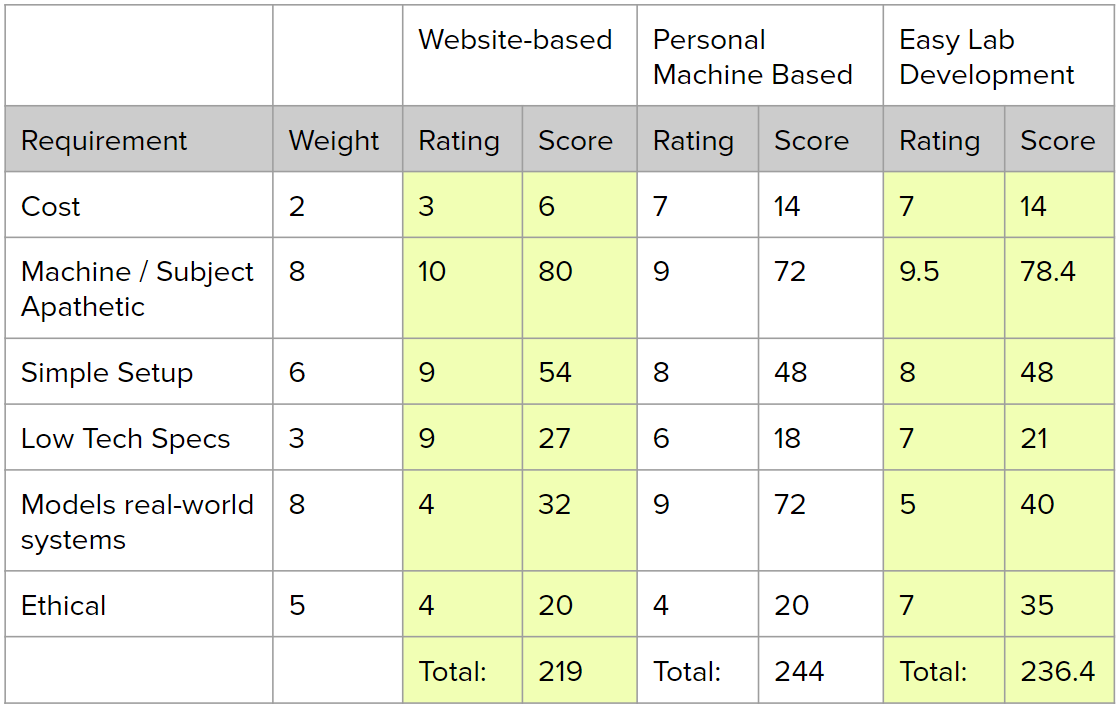
\includegraphics[scale=0.9]{images/IdeaComparison.PNG}
    \captionof{figure}{\textbf{Figure \arabic{figure}:} KTDM chart comparing solution approaches}
\end{center}

\par The personal machine based learning system is our final solution. Website-based learning is too expensive due to hosting costs and fails to accurately model real world systems. However, it had the highest scores for machine apathy, simple setup, and low tech specs due to the user's ability to utilize systems hosted on other computers through a network. The idea of developing labs for professors was similarly weak on its ability to model real world systems due to the high needs of the classroom. If it failed on just one student's computer, it would hold up the whole class or ruin the lesson for the student. And, because there is no way to ensure software works on everyone's machine, this was bound to limit the complexity of the labs we could create\cite{ibrahiminterview}. However, this method was the most ethical due to the ability to have a teacher present encouraging students to use their knowledge ethically. 

\par Ultimately, the personal machine based system won due to its versatility. It can be used to model more complicated systems than the other two solutions because the user has complete control over their machine and needs to wait for no one else. However, it will not be as easy to use due to the lack of an instructor or pre-built systems, and it is not as ethical as classroom teaching. One of the difficulties we will have moving forwards is how to demonstrate attacks and give users experience with penetration testing tools without putting dangerous capabilities in the hands of criminals and angry teenagers. Furthermore, high quality documentation and user testing will be necessary to ensure the setup is intuitive and if any issues arise students have the tools they need to fix them.

\section{Approach}

\par Our group will be taking an Agile/Scrum based approach instead of the traditional Waterfall method for this project. We think our project mission, to enable students to get hands-on experience with penetration testing and security, will benefit from the iterative based project approach. Quick deliverables will enable us to easily reshape our project based on feedback from our professors, industry mentors, and other interested parties. In addition, keeping a regular project velocity will help us get more accomplished in less time and facilitate everyone on our team learning more about development and security. As a result, we hope to be able to end up not only with a finished project at the end of the semester, but a useful tool that will be used and developed by others going forward. More detail on our plans to employ Scrum in the project can be found in our ScrumProposal that we submitted last week.

\section{Conclusion}

\par Software is used everywhere in modern societies, and criminals and governments take advantage of that reliance for nefarious purposes. In order to combat those groups, dedicated software specialists practice cybersecurity. However, there are not enough qualified cybersecurity experts to protect even a fraction of businesses and consumers adequately.

\par Cybersecurity requires a wide domain knowledge due to the complexity of the systems it protects. This makes it hard to learn and dissuades many from pursuing the field. Furthermore, that same complexity makes it difficult to get useful experience with cybersecurity. These two factors combine to create the dire shortage of qualified IT security professionals.

\par We hope to make it easier to model real-world systems by developing a personal machine based solution, likely involving virtualization technology. This should give teachers more tools in the classroom, enable students to get hands-on experience, and generally make the field more approachable. Long term, this could result in more well-trained cybersecurity professionals. 

\par We will go about this development by utilizing the Scrum methodology, where we will complete weekly sprints. At the end of each sprint we will have an actual, deliverable product available for testing. We will integrate feedback on this deliverable from our many resources while implementing new features in a short development cycle such that by the end of the semester we will have a solution to the problem. From there, it will be a matter of ensuring the solution has the necessary impact in the field.


\begin{appendices}
\chapter{Brainstormed Solution Ideas List}

\begin{itemize}
    \item Different basis for education
    \begin{itemize}
        \item Website-based
            \begin{itemize}
                \item Online problems to teach/practice cyber security
                \item Access to services online through SSH/RDP
                    \begin{itemize}
                        \item Domain Controller setup/practice
                        \item Active Directory Training
                        \item Jenkins servers
                        \item WSUS servers
                        \item Tomcat servers
                        \item PhpBB
                        \item NodeJS servers
                    \end{itemize}
                \item Coding challenges through online systems such as codeshare
                \item Online teaching through specific courses and exercises
                    \begin{itemize}
                        \item Potential for monetization
                    \end{itemize}
            \end{itemize}
        \item Personal Machine-based
            \begin{itemize}
                \item Modular system allowing users to download hands-on tutorials 
                    \begin{itemize}
                        \item Modules could demonstrate specific attacks
                            \begin{adjustwidth}{2.5em}{0pt}
                                \begin{enumerate}
                                    \item Silver/Golden Ticket
                                    \item Man in the Middle (MITM)
                                    \item SHA-1 / MD5 Collision Attacks
                                    \item Targeting Kerberos Authentication Protocol
                                    \item Buffer overflow for arbitrary code execution
                                \end{enumerate}
                            \end{adjustwidth}
                        \item Modules could be specifically configured virtual machines
                        \item Modules could be specifically configured programs run on host machine
                        \item Modules could have pre-installed HTML to guide students
                    \end{itemize}
                \item One-time download system
                    \begin{itemize}
                        \item Downloads and installs a system that models a business environment
                        \item Gives students experience in a real environment
                        \item Attacks could be pre-installed
                    \end{itemize}
                \item Either could have a GUI to simplify installation / module selection process
                \item Could have pen testing tools like Metasploit installed
                \item Either could be monetized as a business
                    \begin{itemize}
                        \item Pay for modules or for one-time installation 
                        \item Online market where modules can be developed and sold
                        \item Annual subscription to modules/business services 
                    \end{itemize}
                \item A general framework for encompassing the above
                    \begin{itemize}
                        \item Professors / professionals could utilize and customize
                        \item We could make an implementation to give hands-on pen testing
                        \item Allows easy deployment of IT for non cybersecurity purposes
                    \end{itemize}
                \item Business systems like servers, services, etc. must be installed and configured
                    \begin{itemize}
                        \item Easily deployable business services on any machine, VM or not
                        \item VM's that are specially configured with these services for security use
                    \end{itemize}
            \end{itemize}
        \item Tools for Instructors/deployable labs
            \begin{itemize}
                \item Create easily deployable labs for instructors that are machine apathetic
                \item Make labs to visualize attacks for students
                    \begin{itemize}
                        \item Use virtual Machines, pre-installed software, debugging tools
                        \item Do through text
                        \item Do through code
                        \item Make lab setup guides
                    \end{itemize}
                \item Easily deployable centralized networks and servers to manage labs
                \item Easy scoring system to allow students to compete against each other / professor
                \item Labs that involve attack / defense systems, where two students each take a role
            \end{itemize}
    \end{itemize}
    \item Curriculum Development
        \begin{itemize}
            \item Compare and contrast what content is included in curriculums and degrees globally
            \item See how different study material impacted job security and effectiveness
            \item Build network of professors and interested professionals to develop a curriculum of standards 
            \item Determine how important seeking security extracurriculars is
                \begin{itemize}
                    \item How do we encourage students to engage more in the community?
                \end{itemize}
        \end{itemize}
    \item Alternate and Expanded Possibilities of note
        \begin{itemize}
            \item Outreach and promotion of the field
                \begin{itemize}
                    \item CS outreach to high schools and middle schools
                    \item Introduction and emphasis of application security into more classes within universities
                    \item Hold cheap, easy, hands on CS labs for high school and college students
                    \item Outreach with professors about developing more adversarial labs
                    \item Work to implement basic CS concepts into intro computer science classes, even at the high school level
                    \item CS as play
                        \begin{itemize}
                            \item CS as a competitive sport with audience
                            \item Create easy scoring solutions for adversarial CS competitions to
                                \begin{adjustwidth}{2.5em}{0pt}
                                \begin{enumerate}
                                    \item Makes it easier to set up
                                    \item More competitions
                                \end{enumerate}
                            \end{adjustwidth}
                            \item Simplify and reduce costs of competitions like CCDC
                            \item CS videogames downloadable from windows store/steam
                            \item IoT CS - teach cyber concepts through \$50 toy
                        \end{itemize}
                    \item Start a major CTF for CS and promote it at the high school and college levels
                \end{itemize}
            \item Creating accessibility
                \begin{itemize}
                    \item Implementation solutions
                        \begin{itemize}
                            \item Consolidated documentation on setting up services and labs for practicing CS
                            \item Develop security solutions that can be easily implemented by non-security professionals
                            \item Simplify firewall process: separate firewall config files for different services with ways to combine them
                            \item Simplified logging of key systems on computers
                                \begin{adjustwidth}{2.5em}{0pt}
                                    \begin{enumerate}
                                        \item Powershell on Windows
                                        \item Inbound/Outbound Network Packages
                                        \item Intranetwork packets
                                    \end{enumerate}
                                \end{adjustwidth}
                        \end{itemize}
                    \item Learning solutions
                        \begin{itemize}
                            \item Set up public labs throughout the country
                            \item Khan Academy CS course
                            \item Cloud based systems for portable cybersecurity practice
                            \item Make it seem less intimidating – reduce scope of field fr for new entries into the field
                            \item Business centered around selling virtual CS learning solutions  
                            \item Teaching hardware CS through labs
                            \item Teaching forensics through a modular system
                        \end{itemize}
                \end{itemize}
            \item Broader customer identification
                \begin{itemize}
                    \item Detailed communication with employers about what they need and what they don’t get
                \end{itemize}
        \end{itemize}
\end{itemize}

\end{appendices}

%Sets the bibliography style to UNSRT and imports the 
%bibliography file "samples.bib".

\bibliographystyle{unsrt}
\bibliography{Bibliographies/Phase_I_II.bib}


\listoffigures
\cleardoublepage


\end{document} 